El trabajo con matrices y sus operaciones tiene algunas propiedadess interesantes que nos pueden ser útiles en la solución de problemas de programación competitiva.

\begin{itemize}
	\item Las potencias de una matriz de adyacencia de un grafo tienen una propiedad interesante. Cuando $V$ es una matriz de adyacencia de un grafo no ponderado, la matriz $V^{n}$ contiene la
	número de caminos de $n$ aristas entre los nodos en el grafo.
	\item Usando una idea similar en un grafo ponderado, podemos calcular para cada par de nodos la longitud mínima de un camino entre ellos que contiene exactamente $n$ aristas. Para calcular esto, tenemos que definir la multiplicación de matrices de una manera nueva, de modo que no calculemos el número de caminos sino que minimicemos las longitudes de los caminos. En lugar de la fórmula:
	
	$$  AB[i,j] = \sum_{k=1}^{n}A[i,k]\cdot B[k,j] $$
	
	ahora usamos la fórmula
	
	$$  AB[i,j] = \min_{k=1}^{n}A[i,k] + B[k,j] $$
	
	para la multiplicación de matrices, calculamos un mínimo en lugar de una suma, y una suma de elementos en lugar de un producto. Después de esta modificación, las potencias de la matriz corresponden a los caminos más cortos en el grafo.
	
	\item El teorema de Kirchhoff proporciona una manera de calcular el número de árboles generadores de un grafo como determinante de una matriz especial. Por ejemplo, el grafo: 
	% TODO: \usepackage{graphicx} required
	\begin{figure}[h!]
		\centering
		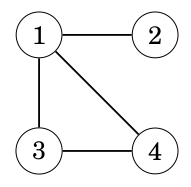
\includegraphics[width=0.15\linewidth]{img/graph_matrix_1}
		\label{fig:graphmatrix1}
	\end{figure}

	tiene tres árboles de expansión:
	
	\begin{figure}[h!]
		\centering
		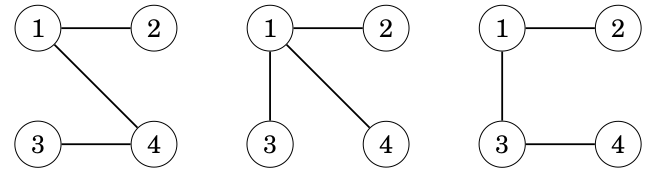
\includegraphics[width=0.5\linewidth]{img/graph_matrix_2}
		\label{fig:graphmatrix2}
	\end{figure}

	Para calcular el número de árboles de expansión, construimos una matriz de Laplacean $L$, donde $L[i,i]$ es el grado del nodo $i$ y $L[i,j]=-1$ si hay una arista entre los nodos $i$ y $j$, y de lo contrario, $L[i,j] = 0$. La matriz de Laplace para el grafo anterior es la siguiente:
	
	$$
	L = \begin{bmatrix}
		3 & -1 & -1 & -1  \\
		-1 & 1  & 0 & 0 \\
		-1 & 0  & 2 & -1 \\
		-1 & 0  & -1 & 2
	\end{bmatrix}
$$	
	Se puede demostrar que el número de árboles generadores es igual al determinante de una matriz que se obtiene cuando eliminamos cualquier fila y cualquier columna de $L$. Por ejemplo, si eliminamos la primera fila y columna, el resultado es:
	
		$$
	det( \begin{bmatrix}
		
		 1  & 0 & 0 \\
		 0  & 2 & -1 \\
		 0  & -1 & 2
	\end{bmatrix}) = 3
	$$
	El determinante es siempre el mismo, independientemente de qué fila y columna
	quitar de $L$ . Tenga en cuenta que la fórmula de Cayley es un caso especial del teorema de Kirchhoff, porque en se aplica a un grafo completo de $n$ nodos.
	
		$$
	det(\begin{bmatrix}
		n-1 & -1 & \ldots & -1  \\
		-1 & n-1  & \ldots & -1 \\
		\vdots & \vdots  & \ddots & \vdots \\
		-1 & -1  & \ldots & n-1
	\end{bmatrix}) = n^{n-2}
	$$	
	
	\item Una recurrencia lineal es una función $f(n)$ cuyos valores iniciales son $f(0),f(1), \dots ,f(k-1)$ y los valores mayores se calculan recursivamente usando la fórmula
	
	$$f(n)= c_1f(n-1)+ c_2f(n-2) + \dots + c_kf(n-k)$$
	
	donde $c_1 , c_2 , \dots , c_k$ son coeficientes constantes.
	
	La programación dinámica se puede utilizar para calcular cualquier valor de $f(n)$ en O($kn$) tiempo calculando todos los valores de $f(0),f(1),\dots ,f(n)$ uno tras otro. Sin embargo, si $k$ es pequeño, es posible calcular $f(n)$ mucho más eficientemente en tiempo O($k^3 \log n$) usando operaciones matriciales.
	
	Un ejemplo sencillo de recurrencia lineal es la siguiente función que define los números de Fibonacci:
	$$\begin{tabular}{rl}
		f (0) = & 0  \\
		f (1) = & 1 \\
		f (n) =	& f ( n - 1) + f ( n - 2)  \\
	\end{tabular}$$ 

En este caso, $k = 2$ y $c_1 = c_2 = 1$.

Para calcular eficientemente los números de Fibonacci, representamos la fórmula de Fibonacci como una matriz cuadrada $X$ de tamaño $2 \times 2$, para la cual se cumple lo siguiente:

$$X \cdot \begin{bmatrix}
	f(i)  \\
	f(i+1) 
\end{bmatrix} = \begin{bmatrix}
f(i+1)  \\
f(i+2) 
\end{bmatrix}$$

Por lo tanto, los valores $f(i)$ y $f(i+1)$ se dan como \emph{entrada} para $X$, y $X$ calcula los valores $f(i+1)$ y $f(i+2)$ a partir de ellos. Resulta que dicha matriz es:

$$X = \begin{bmatrix}
	0 & 1  \\
	1 & 1 
\end{bmatrix}$$

Por ejemplo:

$$ \begin{bmatrix}
	0 & 1  \\
	1 & 1 
\end{bmatrix} \cdot \begin{bmatrix}
f(5)  \\
f(6) 
\end{bmatrix} =\begin{bmatrix}
0 & 1  \\
1 & 1 
\end{bmatrix} \cdot  \begin{bmatrix}
5  \\
8 
\end{bmatrix} = \begin{bmatrix}
8  \\
13 
\end{bmatrix} $$

Por tanto, podemos calcular $f(n)$ usando la fórmula
$$ \begin{bmatrix}
	f(n)  \\
	f(n+1) 
\end{bmatrix} = X^n \cdot \begin{bmatrix}
f(0)  \\
f(1) 
\end{bmatrix} = \begin{bmatrix}
0 & 1  \\
1 & 1 
\end{bmatrix}^n \cdot  \begin{bmatrix}
0  \\
1 
\end{bmatrix} $$

Consideremos ahora el caso general donde f ( n ) es cualquier recurrencia lineal. Nuevamente, nuestro objetivo es construir una matriz X para la cual:
 $$ X \cdot \begin{bmatrix}
 	f ( i )  \\
 	f ( i+1 ) \\
 	\vdots \\
 	f(i+k-1) 
 \end{bmatrix} =   \begin{bmatrix}
 	f(i+1)  \\
 	f(i+2) \\
 	\vdots \\
 	f(i+k) 
 \end{bmatrix} $$
 Tal matriz es
 $$ X = 
 \begin{bmatrix}
 	0      &      1 &      0 &      0 & \ldots & 0  \\
 	0      &      0 &      1 &      0 & \ldots & 0  \\
 	0      &      0 &      0 &      1 & \ldots & 0  \\
 	\vdots & \vdots & \vdots & \vdots & \ddots & \vdots  \\
 	0      &      0 &      0 &      0 & \ldots & 1  \\
 	c_k    & c_{k-1}&c_{k-2} &c_{k-3} & \ldots & c_{1}
 \end{bmatrix}$$
 En las primeras $k-1$ filas, cada elemento es $0$ excepto que un elemento es $1$. Estas filas reemplazan $f(i)$ con $f(i+1)$, $f(i+1)$ con $f(i+2)$, y así en. La última fila contiene los coeficientes de recurrencia para calcular el nuevo valor $f(i+k)$.
 Ahora, $f(n)$ se puede calcular en tiempo O($k^3\log n$) usando la fórmula:
 $$  \begin{bmatrix}
 	f ( n )  \\
 	f ( n+1 ) \\
 	\vdots \\
 	f(n+k-1) 
 \end{bmatrix} = X^n \cdot  \begin{bmatrix}
 f(0)  \\
 f(1) \\
 \vdots \\
 f(k-1) 
\end{bmatrix} $$
\end{itemize}